
\section{Enhancing Bitcoin privacy}
There are basically two approaches for enhancing users privacy in Bitcoin:
\begin{itemize}
  \item Mixing services: they achieve users privacy generally without degrading
  the performance of the system. However, they require absolute trust in a third
  party.
  \item Cryptographic extensions of Bitcoin: extensions of the Bitcoin protocol
  which eliminate the need for trusted third parties but tend to be less efficient
  in terms of performance.
\end{itemize}


%%%%%%%%%%%%%%%%%%%%%%%%%%%
% *** FIRST SUB-SECTION ***
%%%%%%%%%%%%%%%%%%%%%%%%%%%
\subsection{Mixing services} A bitcoin mixing service act as mediators and
provides anonymity by transferring payments from an input set of bitcoin
addresses to an output set of bitcoin addresses, such that is it hard to trace
which input address paid which output address, as schematized in figure
\ref{fig:mixing-service-scheme}. Examples of this kind of mixing services are
Mixcoin and CoinParty. The former relies on a third party can violate users
privacy and steal users’ bitcoins (theft is detected but not prevented), while
the second uses more mixing parties and it is considered secure only if $2/3$ of
the mixing parties are honest.

There is also another kind of mixing services in which the service acts as a
``coin history resetter''. In this case, the user sends to the mixer a certain
amount of bitcoin and a return address and the mixer sends back to the user (to
the specified address) someone else’s coins of the same value. Examples of this
kind of services are BitLaundry and Bitcoin Fog. The problem of these services
is that they do not protect form network-layer attacks since the eventually the
user is the one making payments (instead of the mixing service).

\begin{figure}[!htb]
	\centering
	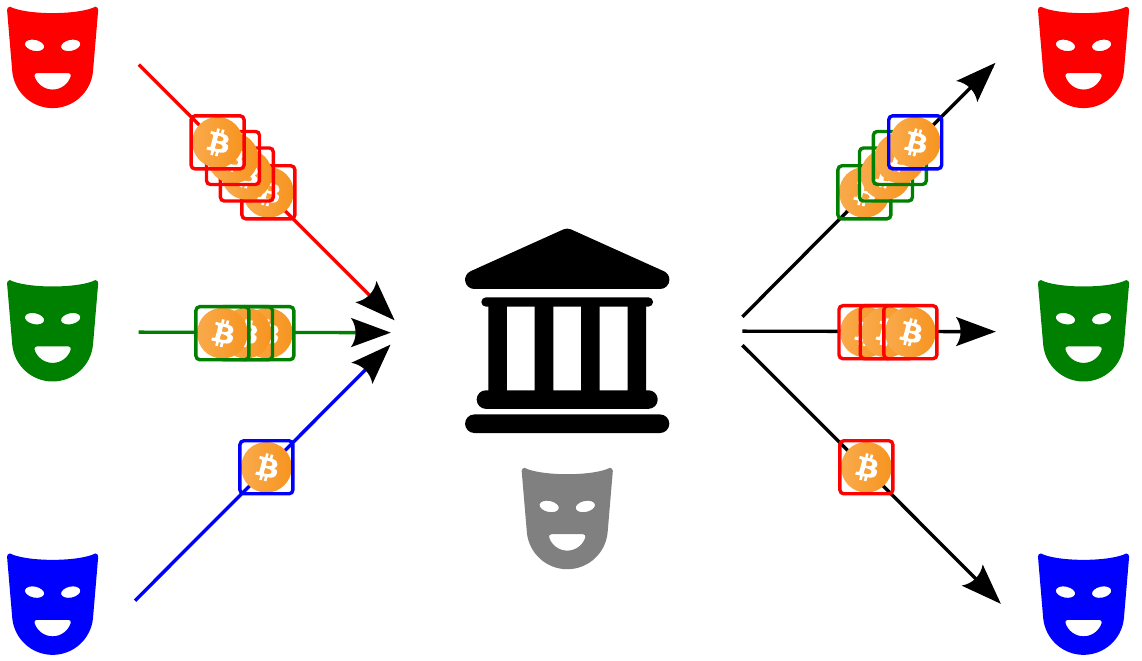
\includegraphics[width=1\linewidth]{img/mixing-service-scheme.png}
	\caption{Scheme of how a mixing service works}
	\label{fig:mixing-service-scheme}
\end{figure}






%%%%%%%%%%%%%%%%%%%%%%%%%%%
% *** SECOND SUB-SECTION ***
%%%%%%%%%%%%%%%%%%%%%%%%%%%
\subsection{Enhancing privacy through blind signatures}\label{sec:enh-sign} In
the following section is presented a mixing service scheme for enhancing Bitcoin
privacy through the use of blind signatures. The scheme has been proposed  by E.
Heilman, F. Baldimtsi and S. Goldberg \cite{heilman-blindly-signed-contracts},
is based on the scheme used in eCash \cite{Chaum1984} and, unlike other previous
schemes that are efficient but achieve limited security/anonymity or other which
provide strong anonymity but are slow and require large numbers of transactions,
it provides anonymity at reasonable speed using an untrusted third party (which
can, therefore, be malicious).

\subsubsection{High-level overview of the scheme}
\paragraph{Scenario}
The scenario is the following: $A$, \emph{the payer}, wants to anonymously send
1 bitcoin to $B$, \emph{the  payee}. If $A$ performed a standard transaction
sending 1 BTC from $address_A$ (owned by $A$) to a fresh ephemeral address
$address_B$ (owned by $B$), there would be a record in the blockchain linking
the two addresses. Even if $A$ and $B$ always create a fresh address for each
payment they receive, the links between addresses can be used to de-anonymize
users when they for example have a transaction with a third party which learns
their identify (e.g. their email address). The basic idea is to used a third
party $I$ that breaks the link between $A$ and $B$ addresses: $A$ sends coins to
$I$ and $I$ sends different coins for the same value to $B$, acting thus as a
mixing service. If other users use $I$ and enough transactions pass through it,
it becomes difficult for an attacker to link $A$ and $B$.

\emph{The main problem is that $I$ knows everything about the transactions between
$A$ and $B$}.

\paragraph{eCash scheme}
A possible solution to this issue is the scheme used in eCash for preventing $I$
from knowing who $A$ wants to pay. This scheme is shown in figure
\ref{fig:eCash-scheme} and relies on blind signatures. $A$ chooses a random
serial number $sn$, blinds it to $\overline{sn}$ and asks $I$ to compute a blind
signature $\overline\sigma$ on $\overline{sn}$, which sends back to $A$. $A$
unblinds these values to obtain $V = (sn, \sigma)$ and then pays $B$ using the
voucher $V$. Finally, $B$ redeems $V$ with $I$ to obtain the bitcoin. With this
scheme $I$ does not know who $A$ wants to pay it cannot read the blinded serial
number $\overline{sn}$ that it signs and it cannot link a message/signature
$(sn, \sigma)$ pair to its blinded value $(\overline{sn}, \overline\sigma)$.
Blindness, therefore, ensures that $I$ cannot link a voucher it redeems with a
voucher it issues. Blind signatures are also unforgeable, which ensures that a
malicious user cannot issue a valid voucher to itself.
\begin{figure}[!htb]
	\centering
	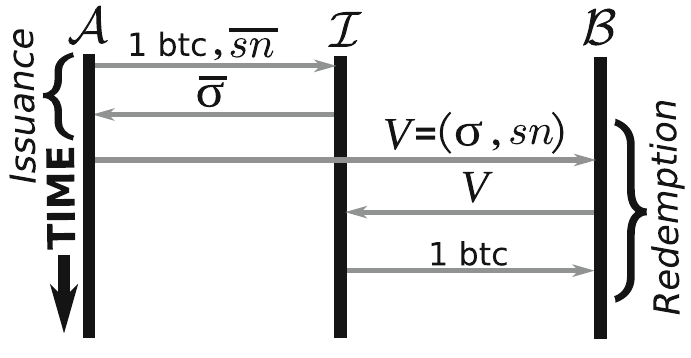
\includegraphics[width=0.6\linewidth]{img/eCash-scheme.png}
	\caption{eCash protocol scheme}
	\label{fig:eCash-scheme}
\end{figure}

\paragraph{Heilman scheme} The main problem with the eCash approach is that $I$
has to be honest: if $I$ is malicious it could refuse to issue a voucher to $A$
after receiving its bitcoin and thus the scheme fails. To solve this, the scheme
proposed in \cite{heilman-blindly-signed-contracts} uses Bitcoin
\emph{transaction contracts} for achieving blockchain-enforced \emph{fair
exchange}. An high-level view of the scheme is shown in figure
\ref{fig:heilman-scheme}. The scheme consists of four blockchain transactions
that are confirmed in three blocks on the blockchain and the key idea is that
$A$ transfers a bitcoin to $I$ if and only if it receives a valid voucher $V$ in
return. The four transactions implement two fair exchanges:
\begin{itemize}
  \item $V\rightarrow BTC$, which consists of the transactions (1) $T_{offer(V\rightarrow
  BTC)}$ and (2) $T_{fulfill(V\rightarrow BTC)}$ and it ensures that a malicious $I$
  cannot redeem $B$’s voucher without providing $B$ with a bitcoin in return.
  The exchange stands in for the interaction between $B$ and $I$.
  Transaction (1) offers a fair exchange of one bitcoin (from $I$) for
  one voucher (from $B$), while transaction (2) is created by $B$ to meet
  the offer by $I$.
  \item $BTC\rightarrow V$, which consists of the two transactions (1) $T_{offer(BTC\rightarrow
  V)}$ and (2) $T_{fulfill(BTC\rightarrow V)}$ and it ensures that a malicious $I$
  cannot take a bitcoin from $A$ without providing it with a voucher $V$.
\end{itemize}


\begin{figure}[!htb]
	\centering
	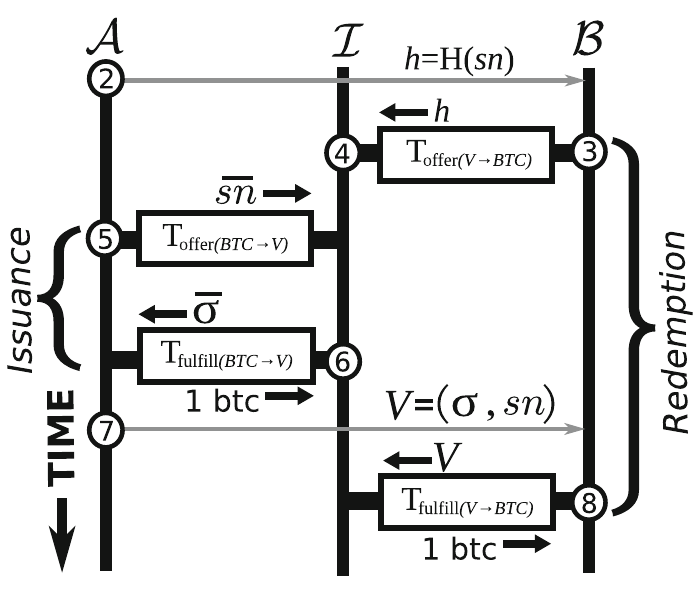
\includegraphics[width=0.6\linewidth]{img/heilman-scheme.png}
	\caption{High-level view of the scheme proposed in \cite{heilman-blindly-signed-contracts}}
	\label{fig:heilman-scheme}
\end{figure}

\subsubsection{Fair exchange implementation} In the following section, it will be
explained how the transaction contracts $T_{offer(BTC\rightarrow V)}$ and (2)
$T_{fulfill(BTC\rightarrow V)}$ implement the fair exchange $BTC\rightarrow V$
used in our protocol scheme shown in figure \ref{fig:heilman-scheme}. The
implementation for the exchange $V\rightarrow BTC$ is analogous.

As already mentioned, the fair exchanges are achieved using transaction
contracts. A transaction contract can be implemented using \emph{Script}, a
simple programming language provided by Bitcoin which, as discussed in chapter
\ref{sec:scripts}, allows to associate each transaction with a script which
defines the rules for spending the transaction outputs, namely how the next
person wanting to spend the bitcoins being transferred can gain access to them.

In this case, the CHECKLOCKTIMEVERIFY feature of Script is used in order to
timelock a transaction, so that funds can be reclaimed if a contract has not
been spent within a given time window $tw$. For implementing the $BTC\rightarrow
V$ fair exchange, $A$ generates the transaction contract
$T_{offer(BTC\rightarrow V)}$ which says the following:

``\emph{$A$ offers bitcoins to $I$ under the condition that $I$ must compute a
valid blind signature on the blinded serial number $\overline{sn}$ (provided by $A$)
within time window $tw$. If this condition is not satisfied, the
bitcoin reverts to $A$.}''

The output of this transaction therefore can be spent in a future transaction $T_f$
only if one of the following conditions is met:
\begin{enumerate}
  \item $T_f$ is signed by $I$ and contains a valid blind signature $\overline\sigma$ on $\overline{sn}$
  \item $T_f$ is signed by $A$ and the time window $tw$ has expired.
\end{enumerate}
For fulfilling the contract and acquiring the bitcoins of the transaction $I$
has therefore to satisfy the condition $2$, which means that $I$ has to post a
transaction $T_{fulfill(BTC\rightarrow V)}$ that contains a valid blind
signature $\overline\sigma$ on $\overline{sn}$. If $I$ does not fulfill the
contract within the time window $tw$, then the condition $2$ is met when $A$
signs and posts a transaction $T_f$ that returns back the offered bitcoins.

\subsubsection{Blind signature scheme} The scheme used for the blind signature
is the Boldyreva’s scheme \cite{boldyreva2003threshold}, which requires two
rounds of interaction. Since the elliptic curve defined by the standard
Secp256k1 used by Bitcoin doesn't support the bilinear pairings required for the
adopted signature scheme, for using the scheme it is necessary to slightly
modify the Bicoin protocol in order to adopt a different elliptic curve.

Let $\mathbb{G}$ be a cyclic additive group of order $p$ (with $p$ prime) in
which the Diffie-Hellman problem is hard and $\mathbb{G'}$ a cyclic
multiplicative group of prime order $q$. Let $e\colon
\mathbb{G}\times\mathbb{G}\to\mathbb{G'}$ be the bilinear pairing, $g$ be a
generator of the group $\mathbb{G}$ and $H$ be a hash function mapping arbitrary
strings to elements of $\mathbb{G}\setminus \{1\}$. The public parameters are
$(p, g, H)$ while the signer public/private key pair is $(sk , pk = g^{sk})$.
The signature scheme works as follow:
\begin{itemize}
  \item To blind $sn$, user $A$ picks random $r\in \mathbb{Z}^{*}_p$ and sets
  $\overline{sn}=H(sn)g^r$.
  \item To sign $\overline{sn}$, signer $I$ computes $\sigma = \overline{sn}^{sk}$.
  \item To unblind the blind signature $\overline{\sigma}$, user $A$ computes
  $\sigma = \overline{\sigma} {pk}^{\-- r}$.
  \item To verify the signature $\sigma$ on $sn$, anyone holding $pk$ checks
  that the bilinear pairing $e(pk,H(sn))$ is equal to $e(g,\sigma)$.
  For verifying the blinded signature $\overline\sigma$ on the blinded
  $\overline{sn}$, anyone holding $pk$ checks if $e(pk,\overline m)= e(g,\overline\sigma)$.
\end{itemize}


\subsubsection{Anonymity considerations} While in the eCash protocol of figure
\ref{fig:eCash-scheme} the anonymity level of users depends on the total number
of payments using $I$, in the scheme proposed by Heilman shown in figure \ref{fig:heilman-scheme} the anonymity level
depends on the number of payment through $I$ in a given epoch. The protocol, in
fact, runs in epochs and provides set-anonymity within each epoch. An epoch is the
three-blocks window in which the four transactions required by the protocol are
confirmed and stored, as shown in figure \ref{fig:epochs}.
\begin{figure}[!htb]
	\centering
	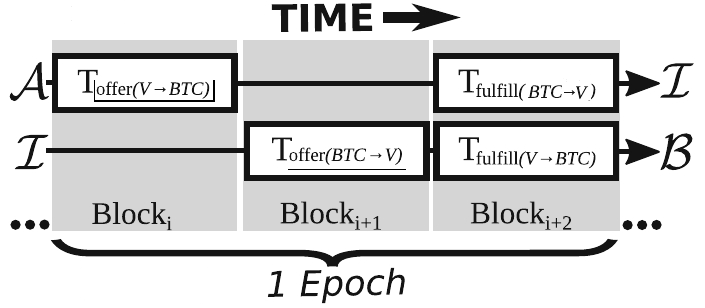
\includegraphics[width=0.6\linewidth]{img/epochs.png}
	\caption{}
	\label{fig:epochs}
\end{figure}

The anonymity considerations about the proposed scheme are based on the following
assumptions:
\begin{itemize}
  \item all the users coordinate on epoch so that the transactions arrangement
  shown in figure \ref{fig:epochs} is respected (e.g. they choose the starting
  block so that its height\footnote{height=distance from the genesis block}
  is multiple of three)
  \item the payer $A$ and the payee $B$ trust each other. If $A$ or $B$ were malicious
  they could easily conspire with $I$ revealing the other part identity: for example
  $A$ could comunicate $I$ the serial number of the received voucher so that when
  $I$ can identify $B$ when he redeems that voucher
  \item payees B always receive payments in a fresh ephemeral address $address_B$
  \item payers only make one anonymous payment per epoch. Similarly, payees only
  accept one payment per epoch.
\end{itemize}

\paragraph{Epoch set-anonymity} As consequence of assumptions (2) and (3), in
every epoch there are exactly $n$ addresses making payments (playing the role of
payer $A$) and $n$ receiving addresses (playing the role of $B$). Anyone looking
at the blockchain can therefore see the participating addresses of payers and
payees, but the probability of successfully linking any chosen payer $A$ to a
payee $B$ should not be more than $1/n$, namely an attacker observing the
blockchain can do no better than randomly guessing who paid whom during an epoch.

\paragraph{Transparency of anonymity} Users learn the size of their anonymity
set (number of participants in their epoch) only after a transaction completes
by looking at the blockchain. If particular $B$ feels his anonymity set is too
small in one epoch, he can increase the size of it by using the scheme as  a
mixing service and making a new transaction to another address owned by him. For
example:  $address_B$ gets paid in an epoch with $n = 4$. $B$ can create a fresh
ephemeral address $address'_B$ and have $address_B$ pay $address'_B$ in a
subsequent epoch. If the subsequent epoch has a $n = 100$, then B increases the
size of his anonymity set.

\paragraph{Intersection attack} As pointed out by the autors in
\cite{heilman-blindly-signed-contracts}, there's the possibility for an attacker
(or anyone looking at the blockchain) to attempt an intersection attack that
de-anonymaze users across different epochs by using frequencial analysis.
